% !TEX root = msc_thesis.tex

\mychapter{2}{Implementation} \label{chap:implementation}


\section{Profs}

ELASPIC uses a domain-based approach for creating homology models of query proteins, and therefore requires accurate domain definitions for all proteins. The most widely-used source of protein domain definitions is Pfam \cite{punta_pfam_2012}. However, since Pfam domains definitions are based entirely on protein sequence, they show a poor correlation with the structural fold of the protein. Using Pfam domain definitions when making homology models would tend to produce unstable structures of split and truncated domains, and this would compromise our subsequent analysis of the structural impact of mutations.

In order to improve the structural accuracy of Pfam domains, Andres Felipe Giraldo Forero developed a pipeline that uses structural alignments and a set of heuristics to modify Pfam domain definitions and make them better aligned with the tertiary structure of the protein, as defined by CATH \cite{cuff_extending_2011}. He named this pipeline Profs, for Protein families. A schematic of this pipeline is presented in Figure \ref{fig:profs_pipeline}, and the R package implementing the pipeline is available at \url{https://bitbucket.org/afgiraldofo/profs}.

Profs combines information from Pfam and CATH in order to improve the accuracy of domain definitions. Profs domains have an advantage over Pfam domains in that they have been corrected and expanded to match the structural fold of the protein. They also have an advantage over CATH domains in that they are backed by large, manually-seeded alignments, and can be easily detected in any protein sequence using Pfam HMMs. We used Andres' pipeline to annotate with Profs domains all proteins in the PDB and UniProt, starting from Pfam domain definitions which we downloaded from SIMAP. The resulting table of Profs domain definitions is available for download from the ELASPIC downloads page: \url{http://elaspic.kimlab.org/static/download/}.

The following sections describes the procedure used to generate lists of Profs domain definitions and Profs domain-domain interactions for all proteins in the PDB and Uniprot.

\begin{figure}[t]
	\centering
	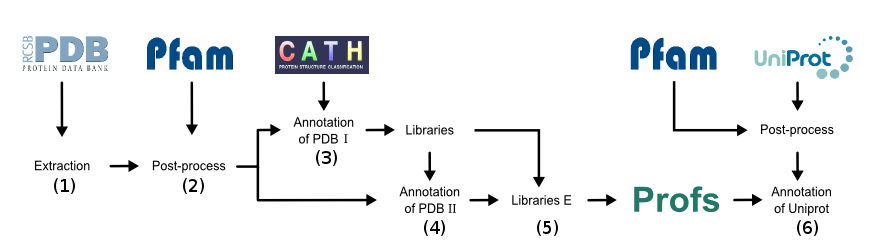
\includegraphics[width=1.0\linewidth]{static/profs/profs_pipeline.png}
	\caption[Flowchart illustrating steps in the Profs pipeline.]{Flowchart illustrating steps in the Profs pipeline (courtesy of Andres Felipe Giraldo Forero). Each step in the flowchart is annotated with the section number where that step is explained. \textbf{(1)} All structures in the PDB are parsed to extract protein sequences, and HMMScan is ran to find Pfam domains in those sequences. \textbf{(2)} Pfam domains of proteins in the PDB are processed in order to join and / or remove overlapping and repeating domains. \textbf{(3)} Pfam domain definitions are altered in order to make them compatible with CATH definitions, for structures that have been annotated by CATH. \textbf{(4)} Pfam domain definitions are altered in order to make them compatible with CATH definitions, for structures that have not been annotated by CATH. This is done by performing pairwise alignments with structures that do have CATH annotations. \textbf{(5)} Libraries of Profs domain definitions, and Profs domain-domain interactions, are generated for all proteins in the PDB.  \textbf{(6)} Libraries of Profs domain definitions, and Profs domain-domain interactions, are generated for all proteins in Uniprot.}
	\label{fig:profs_pipeline}
\end{figure}


\subsection{Domains}

We use Pfam domain definitions calculated for all proteins in the PDB to find Profs domains, and structural templates for those domains, for all proteins in Uniprot. To do this, we follow a similar process to what is done to annotate with Profs domains structures in the PDB that lack CATH annotations.

We start with Pfam domain definitions for all known protein sequences, which we download from the SIMAP website \cite{rattei_simapcomprehensive_2010}. We map those protein sequences to Uniprot using the MD5 hash of each sequence, and we join or remove overlapping and repeating domains using the steps described in Section 1.2. Next, we follow the procedure outlined in Section 1.4 to generate supradomains and to find Profs domain templates. If a suitable template is found, we proceed to do iterative global alignments using Muscle while expanding the domain boundaries of the Pfam domains to match the domain boundaries of the Profs template.  If two Pfam domains are expanded to occupy the same region in the protein, that region is distributed equally between the preceding and the succeeding domains.

The results of this analysis are stored in the \textbf{uniprot\_domain} and the \textbf{uniprot\_domain\_template} tables in the ELASPIC database (Figure \ref{fig:elaspic_database_schema}). The \textbf{uniprot\_domain} table contains all Pfam domains and supradomains that are obtained after removing repeating and overlapping domains and forming supradomains. The \textit{pdbfam\_name} column contains the name of the Profs domain. The \textit{alignment\_def} column contains either the original Pfam domain definitions or, in the case of supradomains, the merged domain definitions of multiple Pfam domains. The \textbf{uniprot\_domain\_template} table contains information describing the alignment of the Pfam domain or supradomain with the corresponding Profs structural template, for domains for which a suitable Profs template could be found. The \textit{cath\_id} column identifies the Profs structural template that was selected, and the \textit{domain\_def} column contains the corrected and expanded domain definitions.

In order to ascertain the validity of Profs domain definitions, we compared Profs, Pfam and Gene3D in terms of sequence coverage (Figure \ref{fig:profs_coverage}) and domain size (Figure \ref{fig:profs_domain_size}).

We downloaded Pfam and Gene3D domain definitions for all human proteins from SIMAP \cite{rattei_simapcomprehensive_2010}, and we calculated Profs domain definitions following the pipeline described above. The analysis was restricted to 18,828 human proteins from UniProt which are annotated with at least one Profs, Pfam or Gene3D domain.

In order to compare sequence coverage, we looked at the fraction of all protein sequences which are covered by each domain type (Figure \ref{fig:profs_coverage}). Overall, Profs has the highest sequence coverage, with 55.7 \% of 10,868,810 amino acids in 18,828 proteins residing inside a Profs domain. Profs annotates ~9 \% more amino acids than Pfam and ~14 \% more amino acids than Gene3D, although the relatively low coverage by Gene3D is expected, as it can only detect domains which are represented in the PDB.

In order to compare domain size, we looked at the average number of domains per protein for each of the three methods (Figure \ref{fig:profs_domain_size}). Profs has more proteins with only one domain per protein, while Pfam and Gene3D have more proteins with two or more domains per protein. This is consistent with Profs trying to join fragmented and repeating domains into consistent structural units. Gene3D does not detect domains in many proteins with Profs and Pfam domains, likely because those domains have not been crystalized.

The result of this analysis shows that, at least for human proteins, Profs achieves higher sequence coverage using fewer domains per protein than either Pfam or Gene3D. This makes Profs well-suited for the ELASPIC pipeline.


\begin{figure}[t]
	\centering
	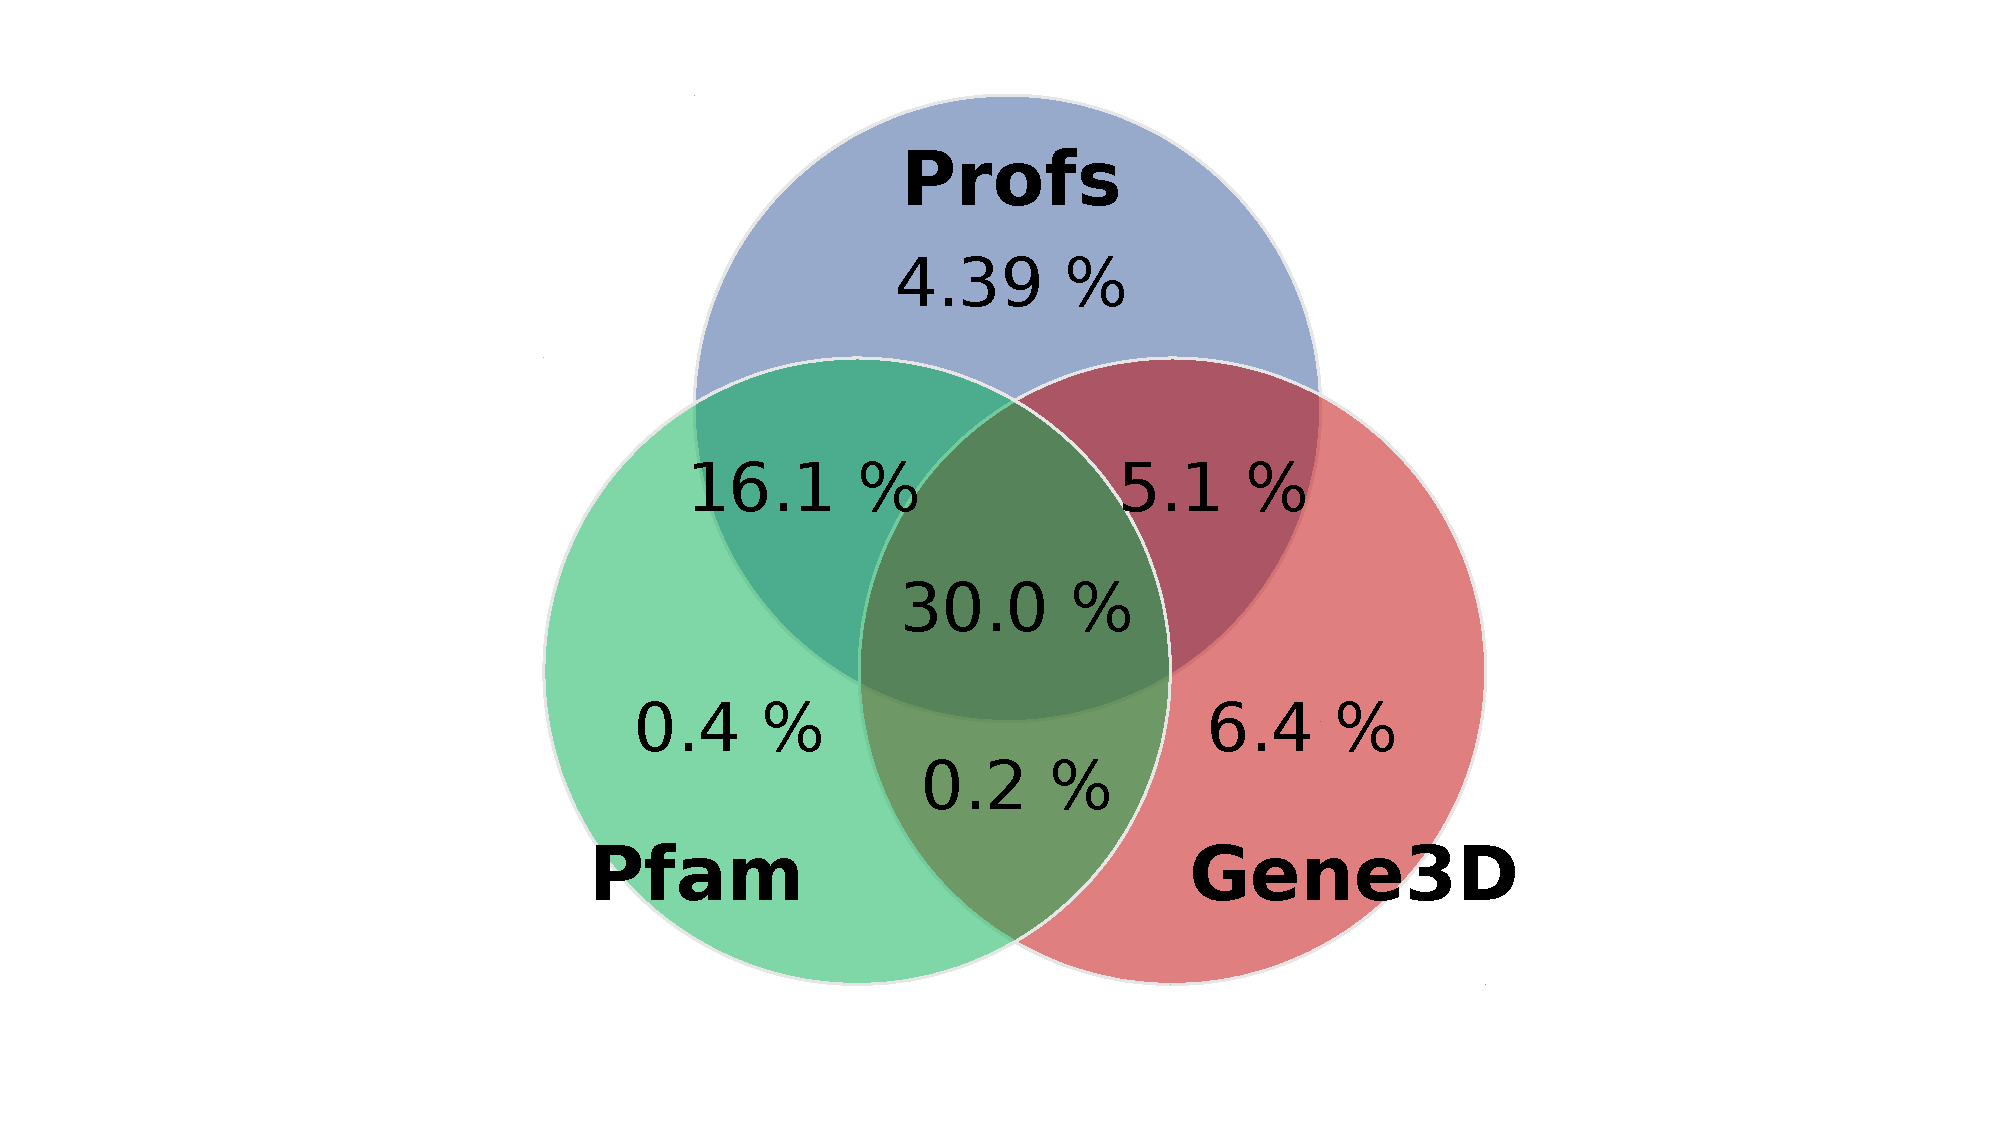
\includegraphics[width=0.7\textwidth]{static/profs/uniprot_coverage_statistics.pdf}
	\caption[Venn diagram showing the overlap in domain definitions between Profs, Pfam, and Gene3D.]{Venn diagram showing the overlap in domain definitions between Profs, Pfam, and Gene3D. Values represent the fraction of amino acids, of all human proteins in UniProt, which are covered the particular domain or domains. A total of 18,828 human proteins and 10,868,810 amino acids were considered, after excluding proteins which had no predicted domains by any method. Profs has the highest coverage, with 55.7 \% of amino acids being annotated by a Prof domain.}
	\label{fig:profs_coverage}
\end{figure}


\begin{figure}[t]
	\centering
	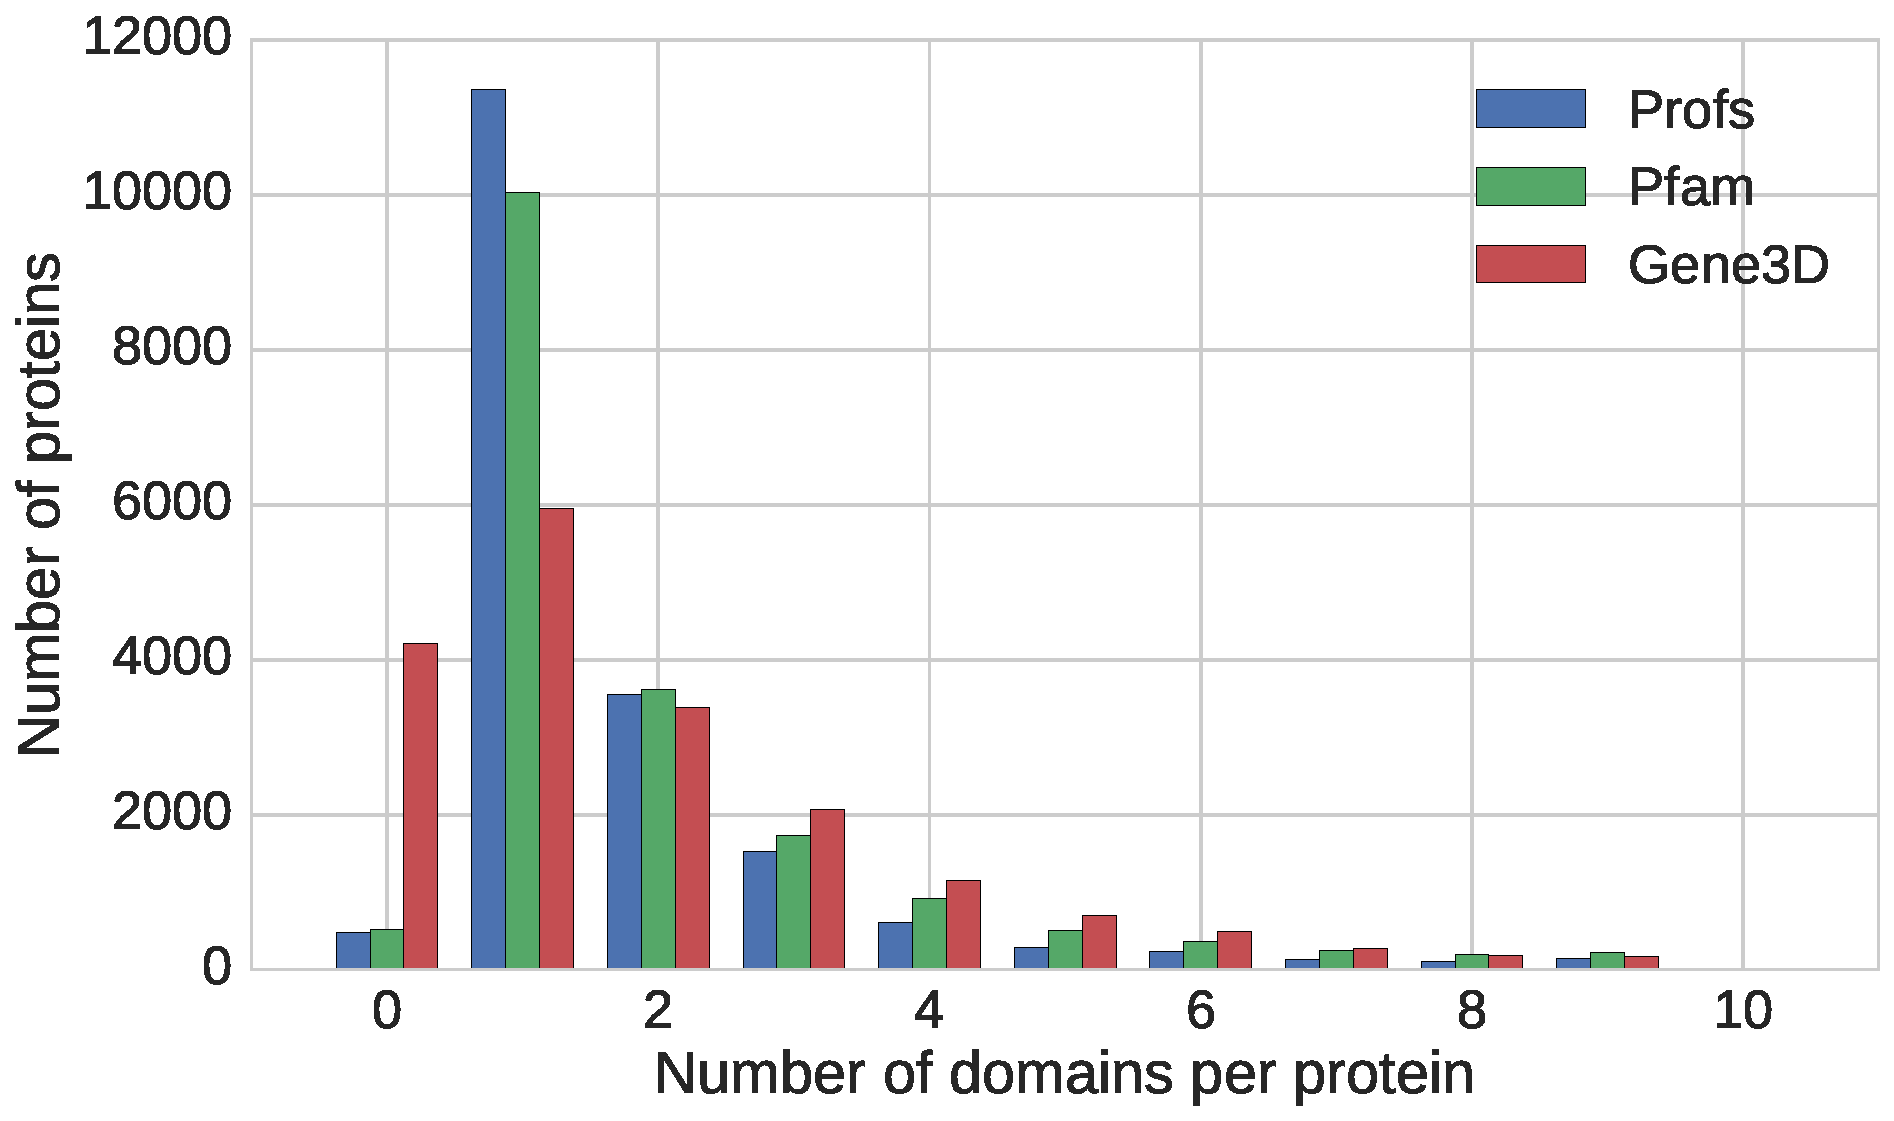
\includegraphics[width=0.9\textwidth]{static/profs/domains_per_protein.pdf}
	\caption[Average number of Profs, Pfam and Gene3D domains per protein]{Average number of Profs, Pfam and Gene3D domains per protein, for all human proteins containing at least one domains. Profs tends to have fewer domains per protein then either Pfam or Gene3D. Gene3D lacks domain annotation for many proteins which contain at least one Pfam and Profs domain.}
	\label{fig:profs_domain_size}
\end{figure}



\subsection{Domain interactions}

We also create a table of domain-domain interactions for proteins that are known to interact and for which a homology model of the interaction can be created. We start by filtering the protein-protein interaction data obtained from HIPPIE \cite{schaefer_hippie:_2012} and all the datasets described in Rolland \textit{et al.} \cite{rolland_proteome-scale_2014} to select pairs of proteins where each protein has at least one domain with a structural template. The overlap in the number of protein-protein interactions described by each dataset is presented in \ref{fig:ppi_database_overlap}. This information is stored in the \textbf{uniprot\_domain\_pair} table. For each of those domains, we perform a Blast search of the domain sequence against a library of Profs domains in the PDB (the \textbf{domain} table, see Figure \ref{fig:elaspic_database_schema}, Table \ref{tab:elaspic_database_schema}), and we select only those templates that occur in the same crystal structure in both proteins and that interact according to the \textbf{domain\_contact} table. In order to select the best template for the interaction, we calculate a quality score for each of the two domains using Equation


\begin{figure}[ht]
	\centering
	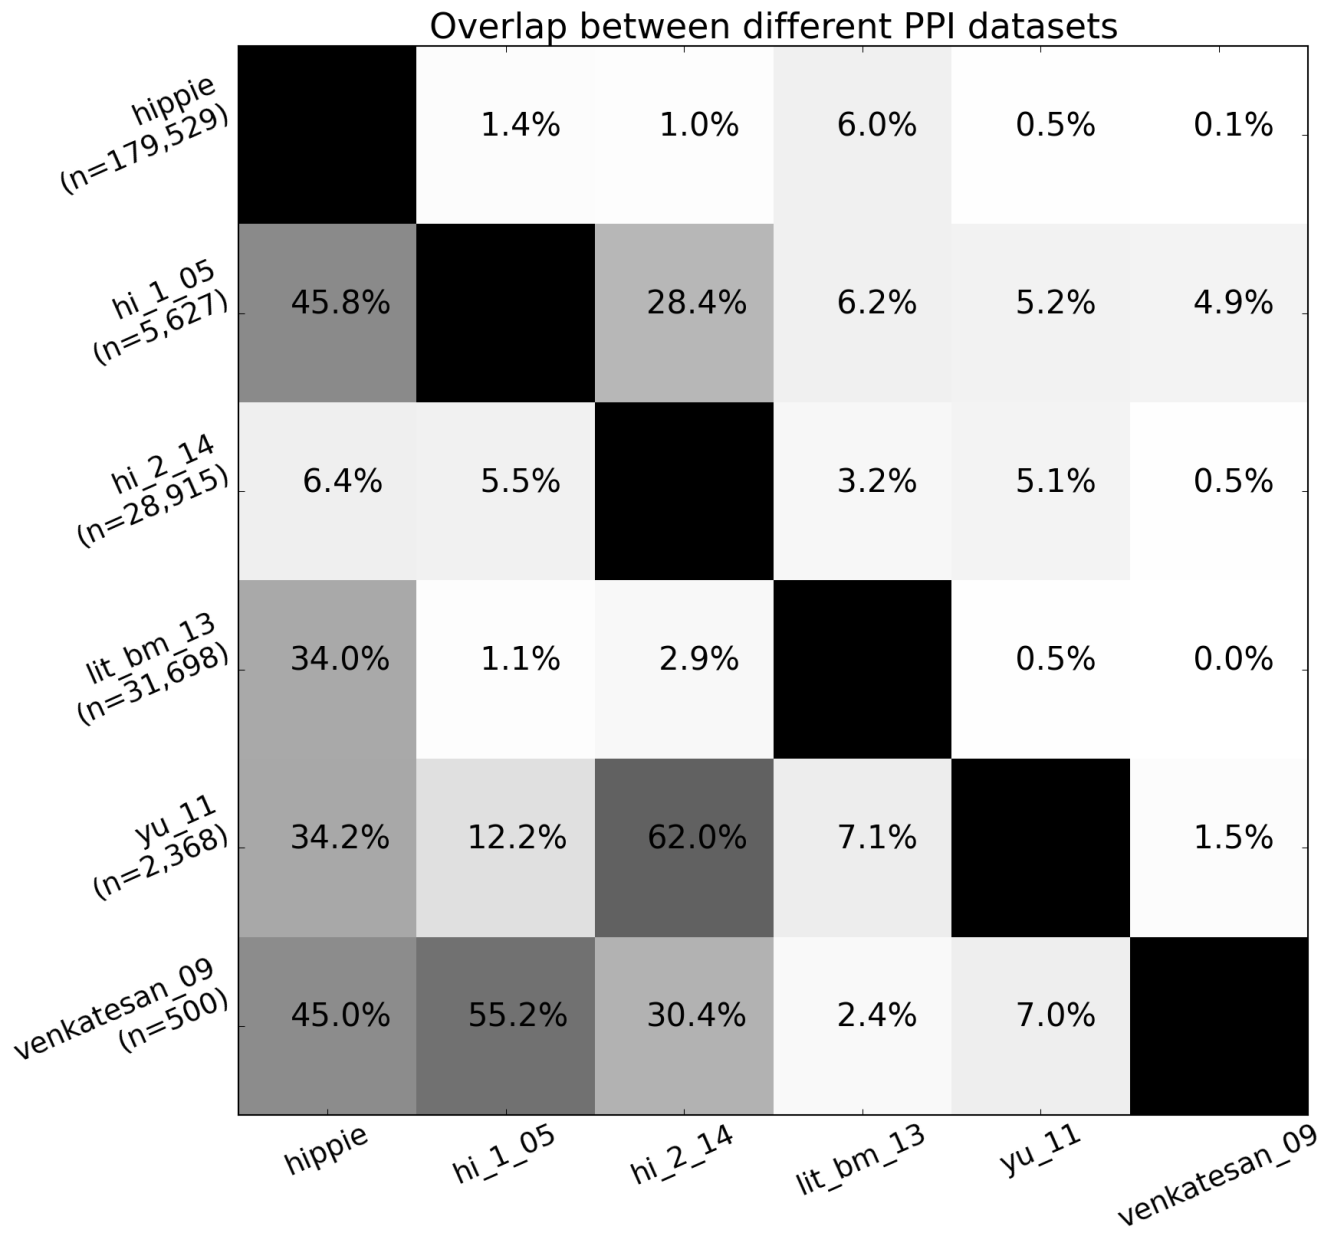
\includegraphics[width=0.6\textwidth]{static/profs/ppi_database_overlap.png}
	\caption[Protein-protein interaction databases.]{Protein-protein interaction databases.}
	\label{fig:ppi_database_overlap}
\end{figure}




\section{ELASPIC}

The ELASPIC project was started by Niklas Berliner and others in 2014 \cite{berliner_combining_2014}.

ELASPIC uses Modeller \cite{webb_comparative_2002} to construct homology models of domains and domain-domain interactions, FoldX to optimize those model and to introduce mutations \cite{schymkowitz_foldx_2005}, and the ELASPIC predictor to combine FoldX energy scores with sequence-based and other features and predict the energetic impact of a mutation on the stability of a single domain or the affinity between two domains. A flowchart describing the ELASPIC pipeline is presented in \ref{fig:elaspic_pipeline}. At each step in the pipeline, a local database is queried to see if the required information has already been calculated. If the information is available, the pipeline moves to the next step. If the information is not available, the pipeline runs the module that generates the required information, stores the generated information in the database for future access, and then moves to the next step. If the specified mutation falls outside of every domain in the protein, no predictions are returned. Otherwise, the pipeline evaluates the impact of the mutation on the stability of the domain and, if the mutation falls in a domain interface, on the affinity between two domains. In order to expedite the evaluation of mutations, we precalculated homology models and Provean supporting sets for all human proteins. Structural and sequential features, and predicted ∆∆G scores, have also been precalculated for the majority of mutations listed in the Uniprot humsavar file \cite{consortium_uniprot:_2015} and in the COSMIC \cite{forbes_cosmic:_2015} and ClinVar \cite{landrum_clinvar:_2016} databases.

Provean supporting sets, homology models and mutation ΔΔG scores are available from the ELASPIC
downloads page: \url{http://elaspic.kimlab.org/static/download/}. The source code of the python package implementing the ELASPIC pipeline is available from \url{https://github.com/kimlaborg/elaspic}, and the documentation for the ELASPIC pipeline can be accessed online at \url{http://elaspic.readthedocs.org}.

\begin{figure}[ht]
	\centering
	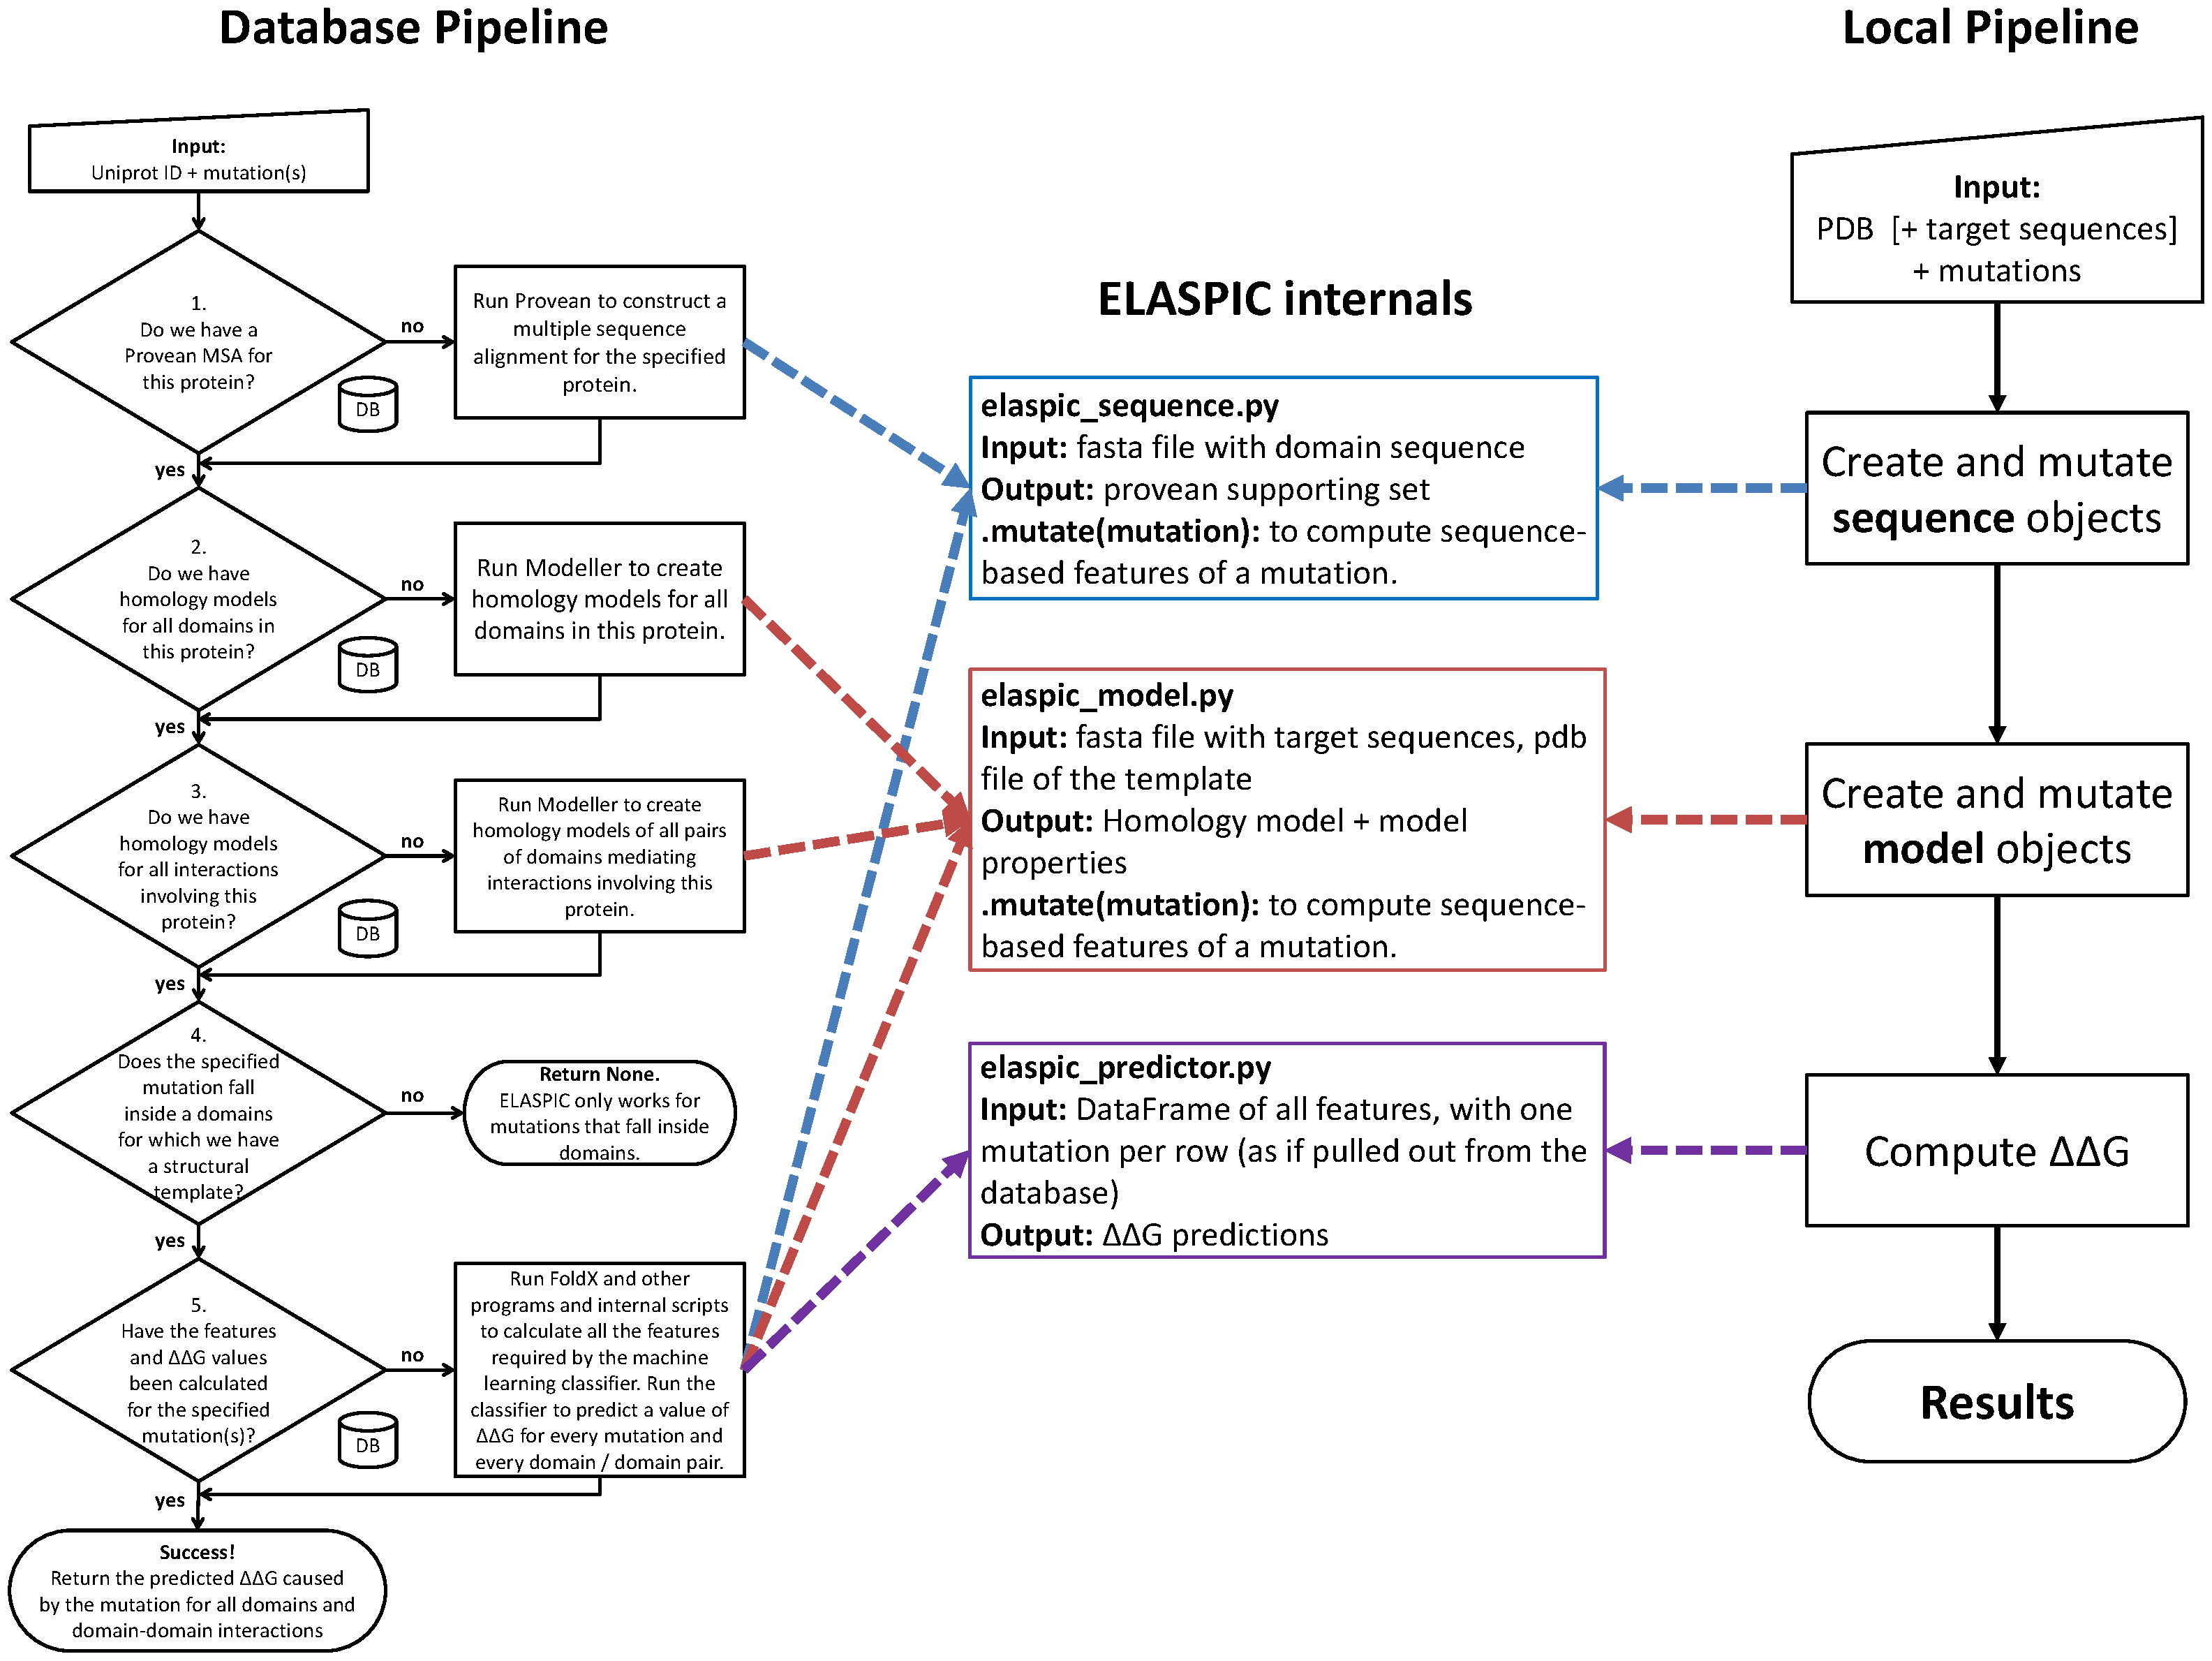
\includegraphics[width=1.0\textwidth]{static/elaspic/elaspic_flowchart.pdf}
	\caption[Overview of the ELASPIC pipeline]{Overview of the ELASPIC pipeline. A user runs the ELASPIC pipeline specifying the UniProt id of the protein being mutated, and one or more mutations affecting that protein. At each decision node, the pipeline queries the database to check whether or not the required information has been calculated previously. If the required data has not been calculated, the pipeline calculates it on the fly and stores the results in the database for later retrieval. The pipeline proceeds until homology models of all domains in the protein, and all domain-domain interactions involving the protein, have been calculated, and the $\Delta \Delta G$ has been predicted for every specified mutation.}
	\label{fig:elaspic_pipeline}
\end{figure}


\subsection{Standalone pipeline}

\ref{fig:elaspic_pipeline} right

An overview of the ELASPIC pipeline is presented in Figure \ref{fig:elaspic_pipeline}. ELASPIC includes a library Python scripts for construction sequence alignments, constructing Provean supporting sets and computing the Provean score, constructing homology models, running FoldX, and predicting the $\Delta \Delta G$ of the mutation. It also includes a ``Standalone Pipeline'' and a ``Database Pipeline'', which include command line options for mutating a protein structure.

The standalone pipeline works without downloading and installing a local copy of the ELASPIC and PDB databases, but requires a PDB structure or template to be provided for every protein. Pipeline output is saves as JSON files inside the working directory, rather than being uploaded to the database as in the case of the database pipeline. The general overview of the local pipleine is presented in the figure to the right.

The local pipeline still requires a local copy of the Blast nr database.

We used the MODELLER software package to perform all homology modeling.

``MODELLER uses simulated annealing cycles along with a minimal forcefield and spatial restraints -- generally Gaussian interatomic probability densities extracted from the template structure with database-derived statistics determining the distribution width—to rapidly generate candidate structures of the target sequence from the provided template sequence.''


\subsection{Database pipeline}

The database pipeline allows mutations to be performed on a proteome-wide scale, without having to specify a structural template for each protein. This pipeline requires a local copy of ELASPIC domain definitions and templates, as well as a local copy of the BLAST and PDB databases.

The general overview of the database pipleine is presented in \ref{fig:elaspic_pipeline} left. A user runs the ELASPIC pipeline specifying the Uniprot ID of the protein being mutated, and one or more mutations affecting that protein. At each decision node, the pipeline queries the database to check whether or not the required information has been previously calculated. If the required data has not been calculated, the pipeline calculates it on the fly and stores the results in the database for later retrieval. The pipeline proceeds until homology models of all domains in the protein, and all domain-domain interactions involving the protein, have been calculated, and the $\Delta \Delta G$ has been predicted for every specified mutation.


\subsection{Database schema}

\begin{figure}[ht]
	\centering
	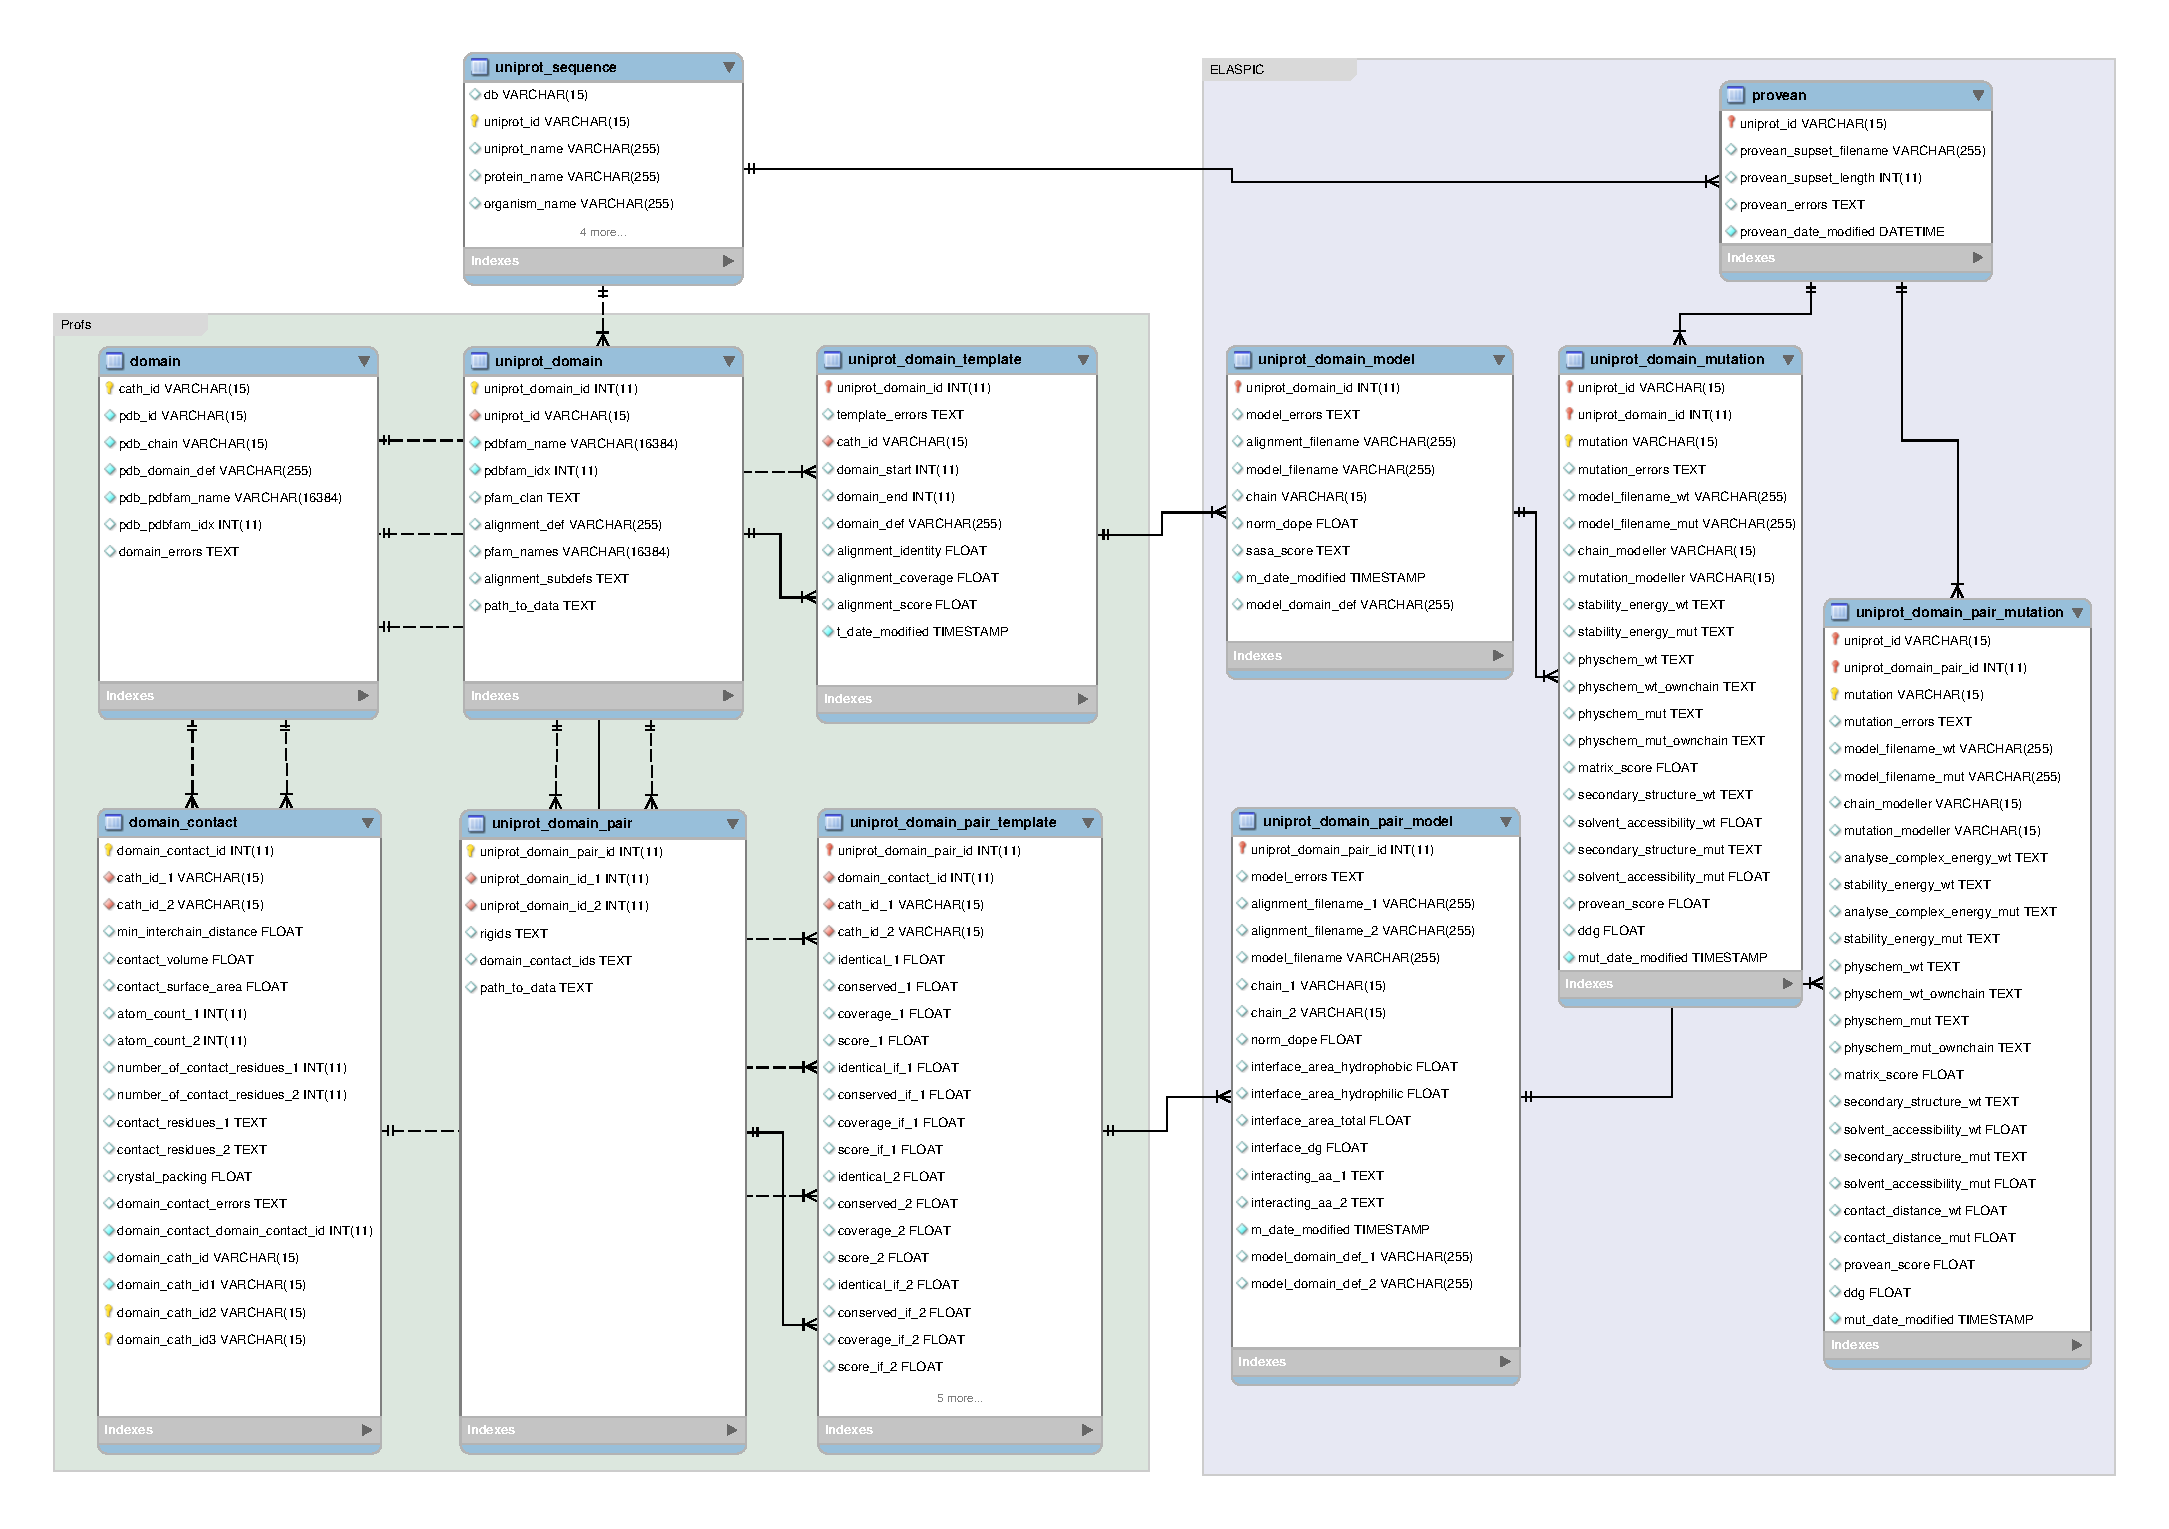
\includegraphics[width=1.0\textwidth]{static/elaspic/elaspic_schema.pdf}
	\caption{Database schema used by the ELASPIC pipeline. Tables on the green plate titled Profs are calculated using the Profs pipeline, as described in \cite{witvliet_elaspic_2016}. Tables on the purple plate titled ELASPIC are calculated using the ELASPIC pipeline, following the procedure outlined in \ref{fig:elaspic_pipeline}. A detailed description of each table can be found in \ref{tab:elaspic_database_schema}.}
    \label{fig:elaspic_database_schema}
\end{figure}


\begin{table}[ht]
\caption{ELASPIC database schema.} \label{tab:elaspic_database_schema}
\begin{tabular}{l | p{10cm}}
	\toprule
	Table name & Table description \\
	\midrule
	\textbf{domain} & Contains Profs domain definitions for all proteins in the PDB. \\
	\textbf{domain\_contact} & Contains information about interactions between Profs domains in the PDB. Only interactions that are predicted to be real by NOXclass \cite{zhu_noxclass:_2006} are included in this table. \\
	\textbf{uniprot\_sequence} & Contains protein sequences for all proteins that are annotated with Profs domains in the \textbf{uniprot\_domain} table. This table is constructed by downloading and parsing \textit{uniprot\_sprot\_fasta.gz}, \textit{uniprot\_trembl\_fasta.gz}, and \textit{homo\_sapiens\_variation.txt} files from the Uniprot. \\
	\textbf{provean} & Contains information about Provean \cite{choi_predicting_2012} supporting set files. The construction of a supporting set is the longest part of running Provean. Thus, in order to speed up the evaluation of mutations, the supporting set is precalculated and stored for every protein. \\
	\textbf{uniprot\_domain} & Contains Profs domain definitions for proteins in the \textbf{uniprot\_sequence} table. This table is obtained by downloading Pfam domain definitions for all known proteins from SIMAP \cite{rattei_simapcomprehensive_2010}, and mapping those proteins to Uniprot using the MD5 hash of each sequence. Overlapping and repeating domains are either merged or deleted, as described in \cite{witvliet_elaspic_2016}. \\
	\textbf{uniprot\_domain\_template} & Contains structural templates for domains in the \textbf{uniprot\_domain} table. The \textit{domain\_def} column contains expanded and corrected domain definitions for every domain. \\
	\textbf{uniprot\_domain\_model} & Contains information about the homology models which were created using structural templates in the \textbf{uniprot\_domain\_template} table. \\
	\textbf{uniprot\_domain\_mutation} & Contains information about the structural impact of core mutations, calculated by introducing those mutations into homology models listed in the \textbf{uniprot\_domain\_model} table. The \textit{ddg} column contains the predicted change in the Gibbs free energy of binding. \\
	\textbf{uniprot\_domain\_pair} & Contains pairs of domains that are likely to mediate the interaction between known interacting partners, obtained from Hippie \cite{schaefer_hippie:_2012} and Rolland et al. \cite{rolland_proteome-scale_2014}. \\
	\textbf{uniprot\_domain\_pair\_template} & Contains structural templates for domain pairs in the \textbf{uniprot\_domain\_pair} table. \\
	\textbf{uniprot\_domain\_pair\_model} & Contains information about homology models which were created using structural templates in the \textbf{uniprot\_domain\_pair} table. \\
	\textbf{uniprot\_domain\_pair} & Contains information about the structural impact of interface mutations, calculated by introducing those mutations into homology models listed in the \textbf{uniprot\_domain\_pair\_model} table. The \textit{ddg} column contains the predicted change in the Gibbs free energy of binding. \\
	\bottomrule
\end{tabular}
\end{table}



\section{Data statistics}

\begin{figure}[ht]
	\centering

	\begin{subfigure}[t]{0.5\textwidth}
		\centering
		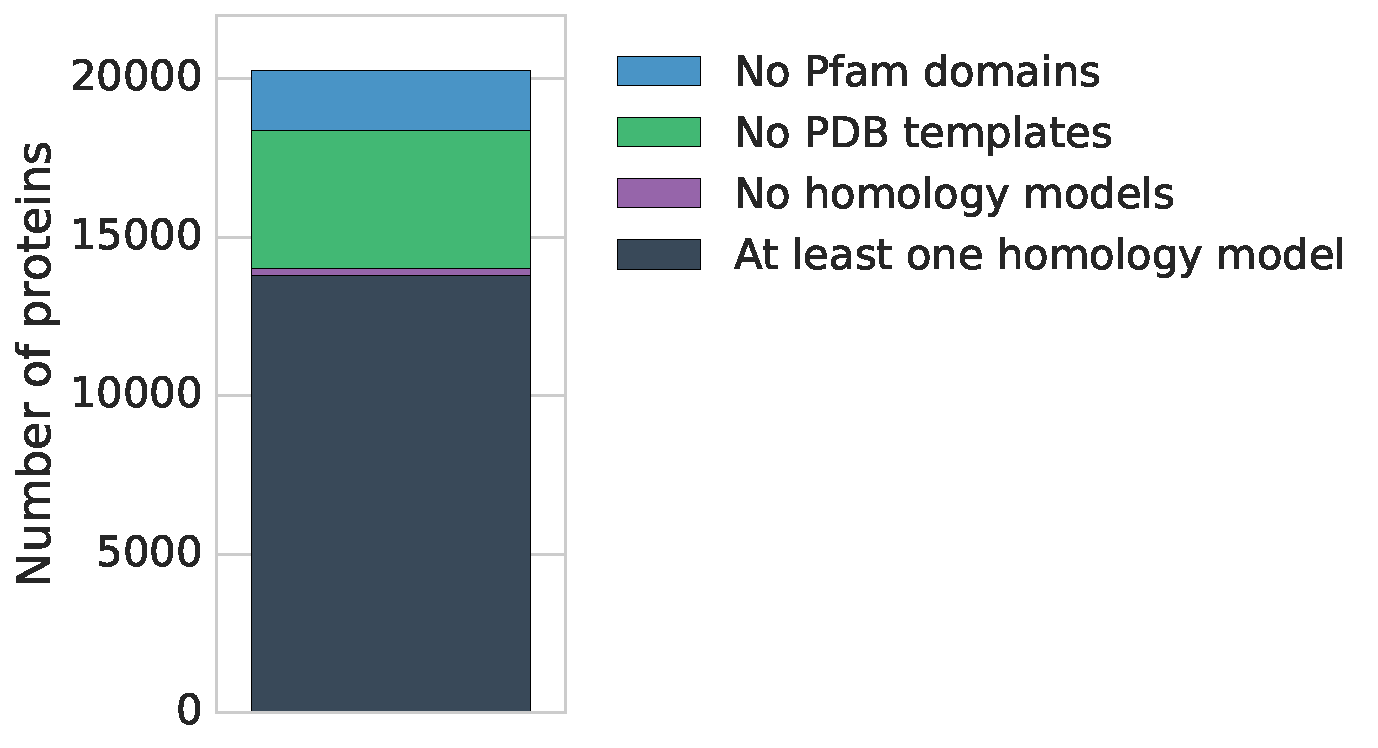
\includegraphics[width=1\linewidth]{static/elaspic_training_set/elaspic_statistics/protein_statistics.pdf}
		\caption{...}
		\vspace*{10mm}
	\end{subfigure}%
	\begin{subfigure}[t]{0.5\textwidth}
		\centering
		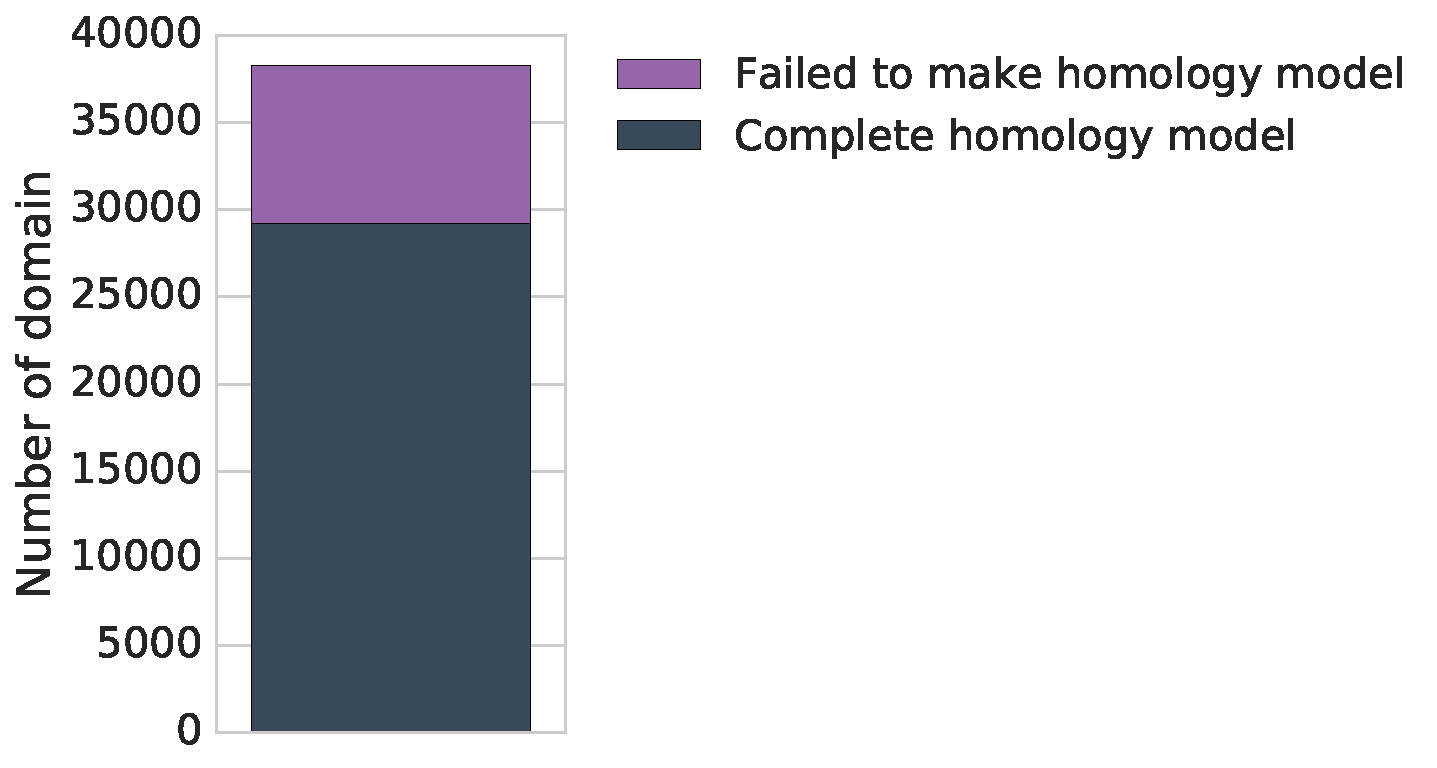
\includegraphics[width=1\linewidth]{static/elaspic_training_set/elaspic_statistics/domain_statistics.pdf}
		\caption{...}
		\vspace*{10mm}
	\end{subfigure}

	\begin{subfigure}{1.0\textwidth}
		\centering
		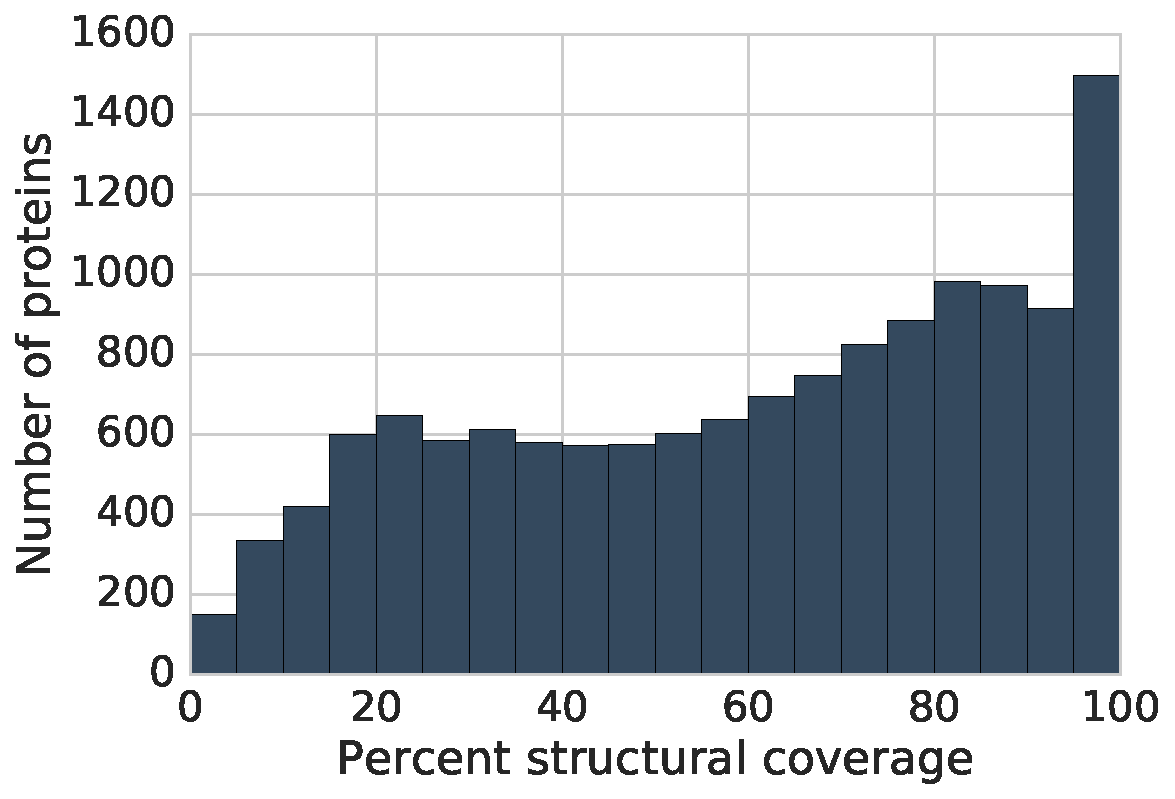
\includegraphics[width=0.55\linewidth]{static/elaspic_training_set/elaspic_statistics/structural_coverage_hist.pdf}
		\caption{...}
	\end{subfigure}%
	\caption{Statistics on homology modelling coverage.}

\end{figure}


\begin{figure}[ht]
	\centering
	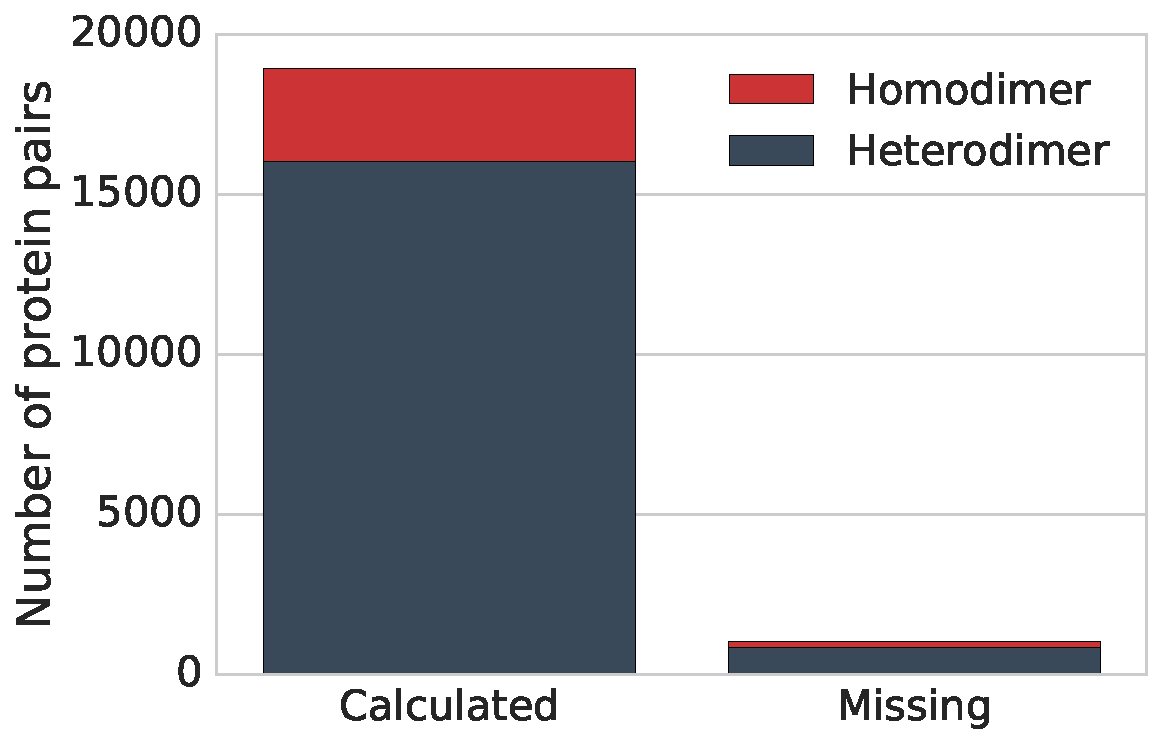
\includegraphics[width=0.4\linewidth]{static/elaspic_training_set/elaspic_statistics/missing_model_protein_pair_novarsplice.pdf}
	\caption{...}
\end{figure}



\subsection{Webservice}

\begin{figure}[ht]
	\centering
	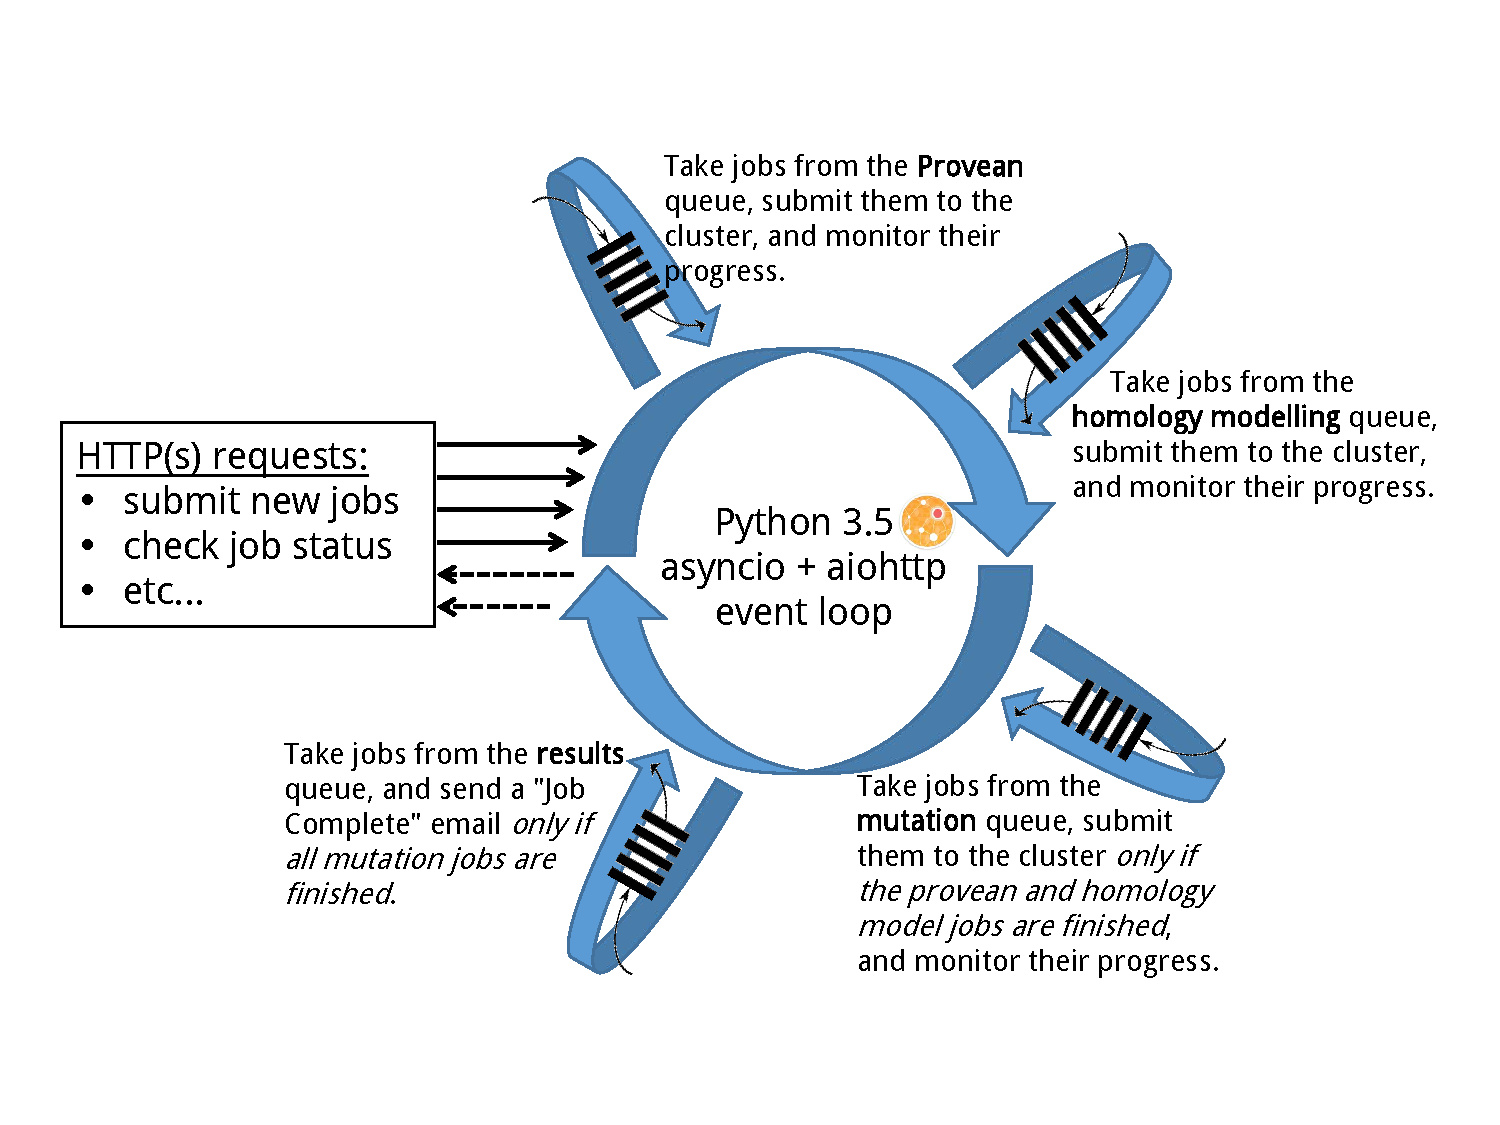
\includegraphics[width=0.8\textwidth]{static/elaspic/elaspic_jobsubmitter.pdf}
	\caption[ELASPIC jobsubmitter]{Overview of the ELASPIC jobsubmitter.}
	\label{fig:elaspic_jobsubmitter}
\end{figure}


\begin{table}[ht]
	\centering
	\caption{ELASPIC web service API.}
	\label{tab:elaspic_jobsubmitter}
	\begin{tabular}{lll}
	\textbf{Method} & \textbf{HTTP request} & \textbf{Description} \\
	submitjob & POST /submitjob & Submit a job to be run on a SGE cluser. \\
	jobstatus & GET /submitjob & View the results of a job.
	\end{tabular}
\end{table}
